\begin{table}
    \centering
        \begin{tabular}{l l l l}
        \toprule
        Setting & NaturalQS & WebQS & TriviaQA \\ 
        \midrule
        RAG (Fine-tuned, Open-Domain) \cite{lewis2020retrieval} & \textbf{44.5} & \textbf{45.5} & \textbf{68.0} \\
        T5-11B+SSM (Fine-tuned, Closed-Book) \cite{roberts2020much} & 36.6 & 44.7 & 60.5 \\ 
        T5-11B (Fine-tuned, Closed-Book) & 34.5  & 37.4 & 50.1 \\
        GPT-3 Zero-Shot & 14.6 & 14.4 & 64.3 \\
        GPT-3 One-Shot & 23.0 & 25.3 & \textbf{68.0} \\
        GPT-3 Few-Shot & 29.9 & 41.5 & \textbf{71.2} \\
        \bottomrule
        \end{tabular}
    \caption{\textbf{Results on three Open-Domain QA tasks.} GPT-3 is shown in the few-, one-, and zero-shot settings, as compared to prior SOTA results for closed book and open domain settings.  TriviaQA few-shot result is evaluated on the wiki split test server.}
    \label{table:question}
\end{table}

\begin{figure}
\vspace{-1em}\centering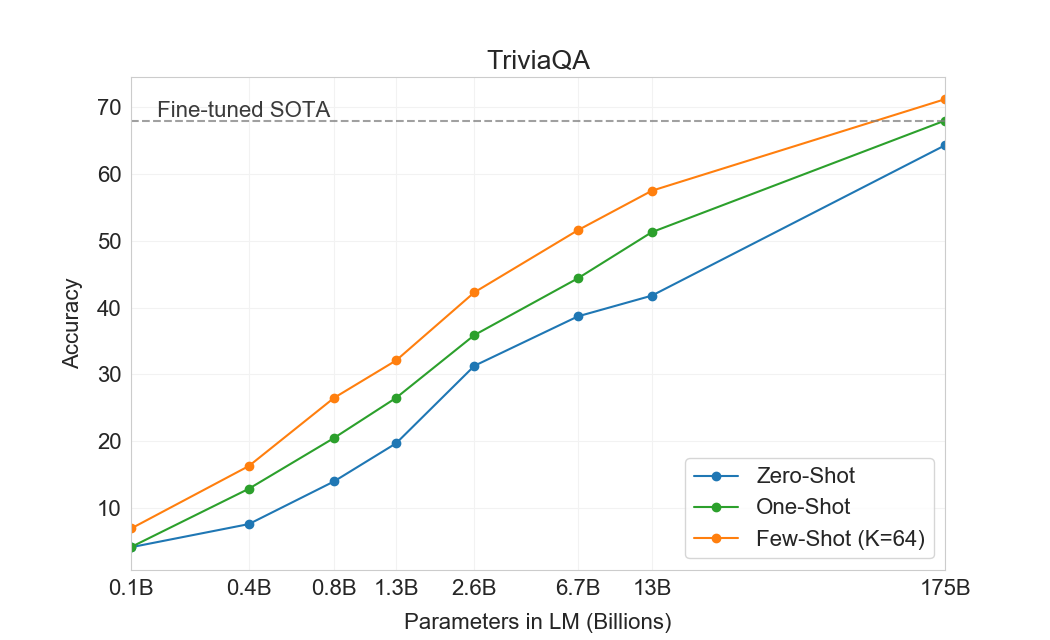
\includegraphics[width=0.8\linewidth]{graphs/scale_plots/triviaqa-wiki.png}
\caption{On TriviaQA GPT3's performance grows smoothly with model size, suggesting that language models continue to absorb knowledge as their capacity increases.  One-shot and few-shot performance make significant gains over zero-shot behavior, matching and exceeding the performance of the SOTA fine-tuned open-domain model, RAG \cite{lewis2020retrieval}}
\label{graph:triviaqa}
\end{figure}

In this section we measure GPT-3’s ability to answer questions about broad factual knowledge. Due to the immense amount of possible queries, this task has normally been approached by using an information retrieval system to find relevant text in combination with a model which learns to generate an answer given the question and the retrieved text. Since this setting allows a system to search for and condition on text which potentially contains the answer it is denoted ``open-book''. \cite{roberts2020much} recently demonstrated that a large language model can perform surprisingly well directly answering the questions without conditioning on auxilliary information. They denote this more restrictive evaluation setting as ``closed-book''.  Their work suggests that even higher-capacity models could perform even better and we test this hypothesis with GPT-3.   We evaluate GPT-3 on the 3 datasets in \cite{roberts2020much}: Natural Questions \cite{Kwiatkowski2019nq}, WebQuestions \cite{berant2013semantic}, and TriviaQA \cite{joshi2017triviaqa}, using the same splits.  Note that in addition to all results being in the closed-book setting, our use of few-shot, one-shot, and zero-shot evaluations represent an even stricter setting than previous closed-book QA work: in addition to external content not being allowed, fine-tuning on the Q\&A dataset itself is also not permitted.

The results for GPT-3 are shown in Table \ref{table:question}. On TriviaQA, we achieve 64.3\% in the zero-shot setting, 68.0\% in the one-shot setting, and 71.2\% in the few-shot setting.  The zero-shot result already outperforms the fine-tuned T5-11B by 14.2\%, and also outperforms a version with Q\&A tailored span prediction during pre-training by 3.8\%.  The one-shot result improves by 3.7\% and matches the SOTA for an open-domain QA system which not only fine-tunes but also makes use of a learned retrieval mechanism over a 15.3B parameter dense vector index of 21M documents \cite{lewis2020retrieval}. GPT-3's few-shot result further improves performance another 3.2\% beyond this.

On WebQuestions (WebQs), GPT-3 achieves 14.4\% in the zero-shot setting, 25.3\% in the one-shot setting, and 41.5\% in the few-shot setting.  This compares to 37.4\% for fine-tuned T5-11B, and 44.7\% for fine-tuned T5-11B+SSM, which uses a Q\&A-specific pre-training procedure.  GPT-3 in the few-shot setting approaches the performance of state-of-the-art fine-tuned models.  Notably, compared to TriviaQA, WebQS shows a much larger gain from zero-shot to few-shot (and indeed its zero-shot and one-shot performance are poor), perhaps suggesting that the WebQs questions and/or the style of their answers are out-of-distribution for GPT-3.  Nevertheless, GPT-3 appears able to adapt to this distribution, recovering strong performance in the few-shot setting.

On Natural Questions (NQs) GPT-3 achieves 14.6\% in the zero-shot setting, 23.0\% in the one-shot setting, and 29.9\% in the few-shot setting, compared to 36.6\% for fine-tuned T5 11B+SSM.  Similar to WebQS, the large gain from zero-shot to few-shot may suggest a distribution shift, and may also explain the less competitive performance compared to TriviaQA and WebQS.  In particular, the questions in NQs tend towards very fine-grained knowledge on Wikipedia specifically which could be testing the limits of GPT-3's capacity and broad pretraining distribution.

Overall, on one of the three datasets GPT-3's one-shot matches the open-domain fine-tuning SOTA. On the other two datasets it approaches the performance of the closed-book SOTA despite not using fine-tuning.  On all 3 datasets, we find that performance scales very smoothly with model size (Figure \ref{graph:triviaqa} and Appendix \ref{appendix:results_on_all_tasks} Figure \ref{graph:all_qa}), possibly reflecting the idea that model capacity translates directly to more ‘knowledge’ absorbed in the parameters of the model.



